%卒業論文概要テンプレート ver. 1.0

\documentclass[uplatex,twocolumn,dvipdfmx]{jsarticle}
\usepackage[top=22mm,bottom=22mm,left=20mm,right=20mm]{geometry}
\setlength{\columnsep}{15mm}
\usepackage[T1]{fontenc}
\usepackage{txfonts}
\usepackage{wrapfig}
\usepackage[expert,deluxe]{otf}
\usepackage[dvipdfmx,hiresbb]{graphicx}
\usepackage[dvipdfmx]{hyperref}
\usepackage{pxjahyper}
\usepackage{secdot}

\makeatletter
\renewcommand{\section}{%
  \@startsection{section}{1}{\z@}%
  {0.6\Cvs}{0.4\Cvs}%
  {\normalfont\normalsize\raggedright}}
\renewcommand{\subsection}{\@startsection{subsection}{2}{\z@}%
  {\z@}{\z@}%
  {\normalfont\normalsize}}
\renewcommand{\subsubsection}{\@startsection{subsubsection}{3}{\z@}%
  {\z@}{\z@}%
  {\normalfont\normalsize}}
\makeatother
%ここから上を編集する必要はない.





%タイトルと学生番号,名前だけ編集すること
\title{\vspace{-5mm}\fontsize{14pt}{0pt}\selectfont Twitterにおけるユーザープロフィールと拡散力の関係分析}
\author{\normalsize プロジェクトマネジメントコース・ソフトウェア開発管理グループ 矢吹研究室 1142016 井上 乃祐}
\date{}
\pagestyle{empty}
\begin{document}
\fontsize{10.5pt}{\baselineskip}\selectfont
\maketitle





%以下が本文
\section{序論}
Twitterは2006年に開始したサービスで,コミュニケーションツールのひとつとして利用されているソーシャル・ネットワーキング・サービスである.国内ユーザーは2014年6月では1980万人,2015年5月では2390万人であり,月間アクティブ率は70.2%である\cite{twitter}.

Twitterはツイートと呼ばれる140字以内の短い文字列を投稿するサービスである.自分以外のユーザーのツイートを読むためには,そのユーザーのページにアクセスする方法以外に,そのユーザーをフォローすることでツイートを読むことができる.フォローしているユーザーのツイートはまとめられ,タイムラインを形成する.

そのほかの機能にリツイート呼ばれるものがあり,それは他の人のツイートを再びツイートするというものである.自分の画面上に流れてきたツイートをリツイートすると,自分のフォロワーの画面にも流れる.同じように,自分がフォローしているユーザーがリツイートすれば,自分のタイムライン上にリツイートが流れてくる.リツイートされるツイートには,ツイート内容という情報以外にアイコンや,ユーザーのIDなどの本質以外の情報も含まれる.

Twitterを利用していると,フォローしているユーザーからリツイートが流れてくることがある.その流れてきたリツイートを見てみると,似たような内容でもリツイートされた回数に違いがあることに気づいた.そこで私はプロフィールのアイコンがリツイート率に影響があるのではないかと考えた.







\section{目的}

Twitterのアイコンが拡散力に影響があるかを調べ,情報の本質でないアイコン部分が本質に与える影響を調べる.

\section{手法}


VirtualBoxをインストールして仮想マシンを作成し,そこにUbuntuをインストールする.その後,Ubuntu上でPythonとTweepyをインストールして,Streaming APIを使用するプログラムを実行し,リツイートされたツイートを集める.

その後,リツイートされたツイートのアイコンをいくつかのタグで分類し,Rを用いて重回帰分析をする.

\begin{figure}[htbp]

\centering
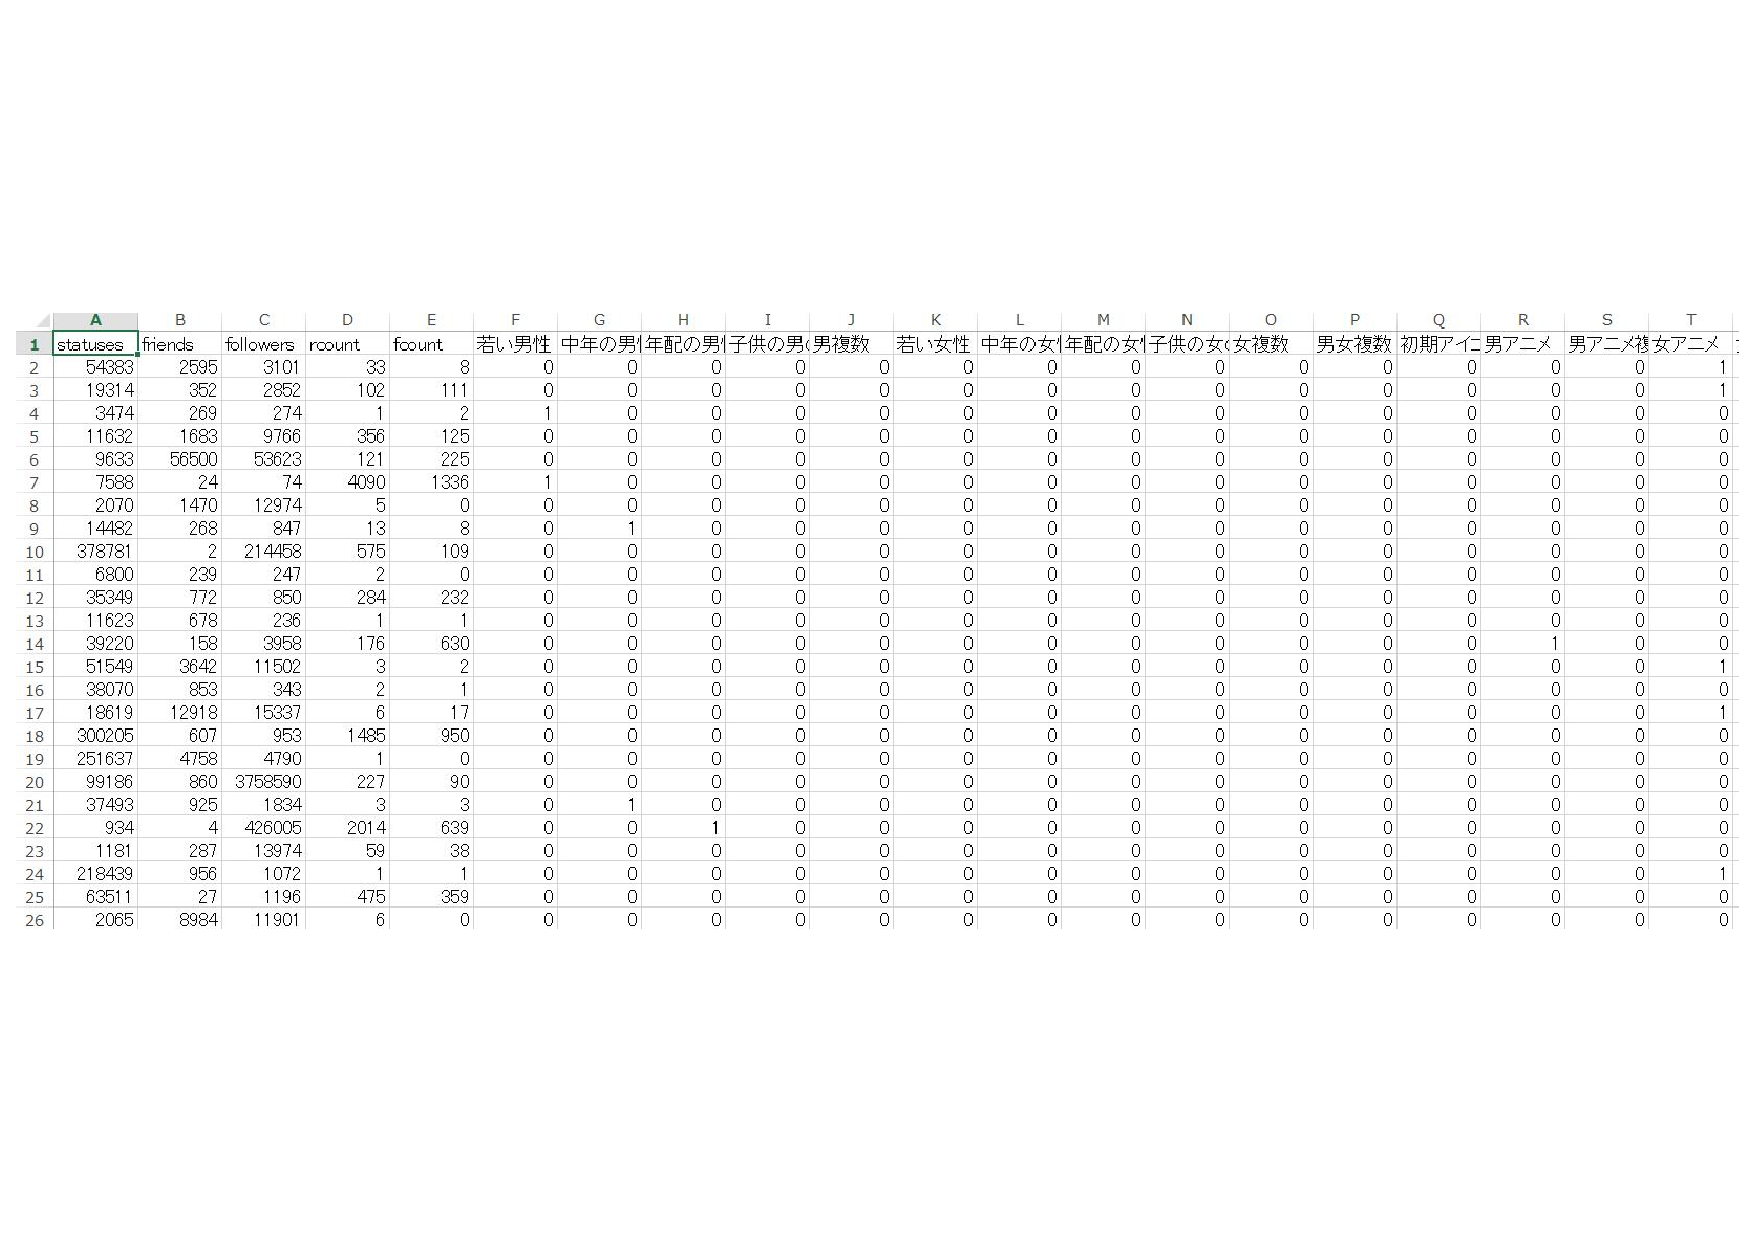
\includegraphics[width=4cm,clip]{exel.pdf}
\caption{収集したデータ}
\label{figure}

\end{figure}
%\bigskip


\section{結果}

若い男性,中年の男性,子供の男の子のタグをつけたアイコンが多くリツイートされている.





\section{考察}

上記の結果を見ると,若い男性,中年の男性,子供の男の子のタグをつけたアイコンが多くリツイートされていた.そこから男性のアイコンのほうが,ツイートに信頼感や,説得力があるからではないかと考えた.

\section{結論}

Twitterでは男性のアイコンのほうがリツイートされる割合が高いと言う結論がでた.



\bibliographystyle{junsrt}
\bibliography{biblio}%「biblio.bib」というファイルが必要.

\end{document}
